\documentclass[tikz, border=3mm]{standalone}
\usepackage{tikz}
\usetikzlibrary{shapes.geometric, arrows.meta, positioning}
\usepackage{fontspec}
\setmainfont{Times New Roman}
\begin{document}
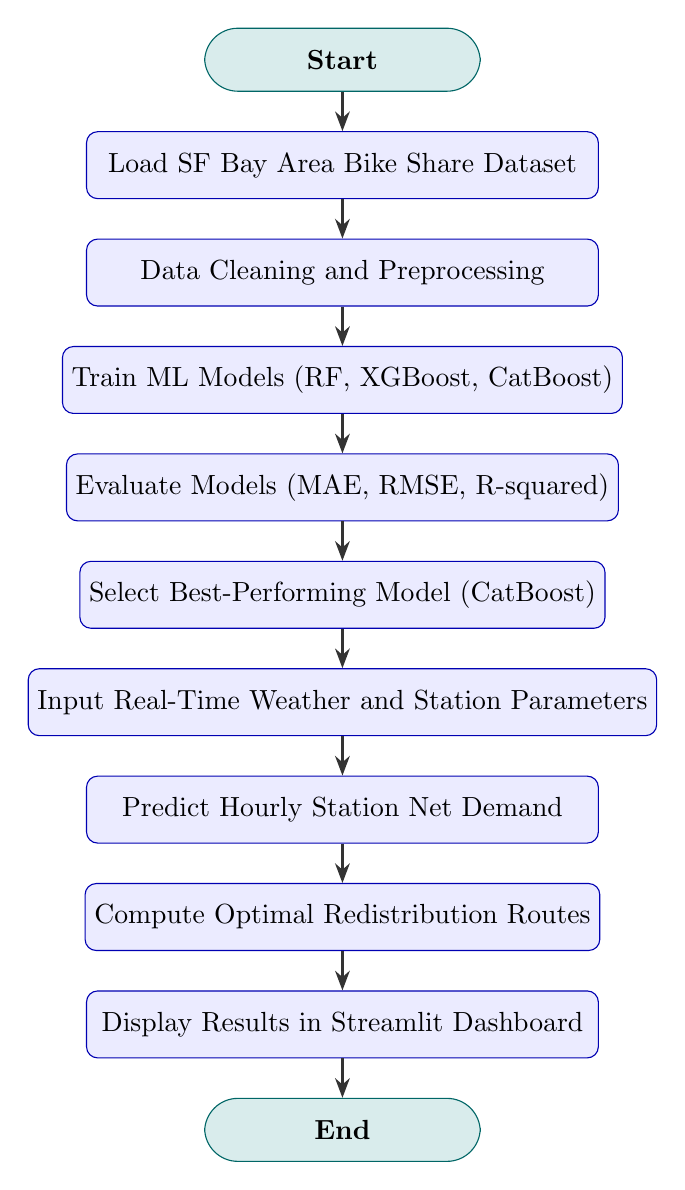
\begin{tikzpicture}[
    startstop/.style={rectangle, rounded corners=12pt, minimum width=3.5cm, minimum height=0.8cm, align=center, draw=teal!80!black, fill=teal!15, font=\rmfamily\bfseries\normalsize},
    proc/.style={rectangle, rounded corners=4pt, minimum width=6.5cm, minimum height=0.85cm, align=center, draw=blue!70!black, fill=blue!8, font=\rmfamily\normalsize},
    arrow/.style={thick, -{Stealth[length=2.5mm]}, draw=black!80}
]

\node (start) [startstop] {Start};
\node (load) [proc, below=0.5cm of start] {Load SF Bay Area Bike Share Dataset};
\node (prep) [proc, below=0.5cm of load] {Data Cleaning and Preprocessing};
\node (train) [proc, below=0.5cm of prep] {Train ML Models (RF, XGBoost, CatBoost)};
\node (eval) [proc, below=0.5cm of train] {Evaluate Models (MAE, RMSE, R-squared)};
\node (best) [proc, below=0.5cm of eval] {Select Best-Performing Model (CatBoost)};
\node (input) [proc, below=0.5cm of best] {Input Real-Time Weather and Station Parameters};
\node (pred) [proc, below=0.5cm of input] {Predict Hourly Station Net Demand};
\node (redist) [proc, below=0.5cm of pred] {Compute Optimal Redistribution Routes};
\node (dash) [proc, below=0.5cm of redist] {Display Results in Streamlit Dashboard};
\node (end) [startstop, below=0.5cm of dash] {End};

\draw [arrow] (start) -- (load);
\draw [arrow] (load) -- (prep);
\draw [arrow] (prep) -- (train);
\draw [arrow] (train) -- (eval);
\draw [arrow] (eval) -- (best);
\draw [arrow] (best) -- (input);
\draw [arrow] (input) -- (pred);
\draw [arrow] (pred) -- (redist);
\draw [arrow] (redist) -- (dash);
\draw [arrow] (dash) -- (end);

\end{tikzpicture}
\end{document}
